\chapter{The SEXTANTE history manager}

\section {Introduction}

Every time you execute a SEXTANTE algorithm, information about the process is stored in the SEXTANTE history manager. Along with the parameters used, the date and time of the execution are also saved.

This way, it is easy to track the and control all the work that has been developed using SEXTANTE, and easily reproduce it.

The SEXTANTE history manager is a set of registries grouped according to their date of execution, making it easier to find information about an algorithm executed at any particular moment.

\begin{center}
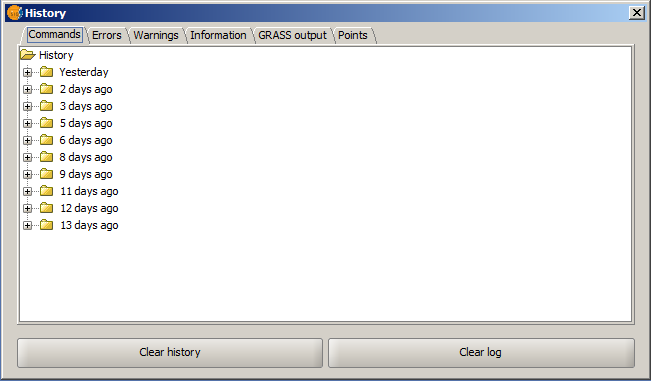
\includegraphics[width=.4\columnwidth]{history.png}
\end{center}

Process information is kept as a command--line expression, even if the algorithm was launched from the toolbox. This makes it also useful for those learning how to use the command--lin interface, since they can call an algorithm using the toolbox and then check the history manager to see how that same algorithm could be called from the command line.

Apart from browsing the entries in the registry, processes can be re--executed, simply double--clicking on the corresponding entry.

You can also right click on a process (the command--line sentence must start with ``runalg'') and select \emph{Open algorithm dialog}. This will show the dialog used to execute the algorithm, already filled with the parameter values corresponding to the selected command.